%
%  Vincent Yannello
%
\documentclass[12pt,fullpage]{article}
\usepackage{fullpage}
\usepackage{amsmath}
\DeclareMathOperator{\erf}{erf}
\usepackage{psfrag}                                          % LaTeX graphics tool
\usepackage{pslatex}                                         % avoids the default cmr font
\usepackage{graphicx}                                        % graphics package 
\usepackage{epsfig}                                          % figures
\usepackage{hyperref}
\usepackage{color}

\begin{document}

\noindent
{\bf Normal distribution} (from \color{blue}\url{http://www.math.wm.edu/~leemis/chart/UDR/UDR.html}\color{black})

\noindent
The shorthand $X \sim {\rm N}(\mu, \sigma^2)$ is used to indicate that the
random variable $X$ has the normal distribution with parameters $\mu$ and $\sigma^2$.
A normal random variable $X$ with mean $\mu$ and variance $\sigma^2$ has probability density function 
$$
f(x) = \frac{1}{\sqrt{2 \pi} \sigma} e^{-{\frac { \left( x-{\it \mu} \right) ^{2}}{{{
2 \it \sigma}}^{2}}}} \qquad \qquad -\infty < x < \infty,
$$
for $-\infty < \mu < \infty$ and $\sigma >0$.
The normal distribution can be used for modeling adult heights, newborn baby weights, ball bearing
diameters, etc. 
The normal distribution can be used to approximate the binomial distribution when $n$ is large
and $p$ is close to $1/2$.
The normal distribution can also be used to approximate the Poisson distribution when $n$ is large
and $p$ is small. 
The central limit theorem indicates that the normal distribution is
useful for modeling random variables that can be thought of as a sum
of several independent random variables.
The probability density function for $\mu = 3$ and two different values of $\sigma$ is illustrated below.

{\begin{figure}[h!]
\begin{center}
\psfrag{lab1}{$\sigma = 1$}
\psfrag{lab2}{$\sigma = 2$}
\psfrag{labx}{$x$}
\psfrag{labf}{$f(x)$}
\includegraphics[width=3.2in]{NormalPlot.ps}
\end{center}
\end{figure}}

\noindent
The cumulative distribution function on
the support of $X$ is
$$
F(x) = P(X \le x) = \frac{{\it \erf} \left({\frac { x-{\it 
\mu}}{{\sqrt{2} \it \sigma }}} \right)+1}{2}  \qquad \qquad -\infty < x < \infty,
$$
where
$$
\erf(x) = \frac{2}{\sqrt{\pi}}\int_0 ^x e^{-{t^2}}dt \qquad \qquad x > 0
$$
and $\erf(-x) = -\erf(x)$.
The survivor function on the support of $X$ is
$$
S(x) = P(X \ge x) = \frac{1 - {\it \erf} \left({\frac { x-{\it 
\mu}}{{\sqrt{2} \it \sigma }}} \right)}{2}  \qquad \qquad -\infty < x < \infty.
$$
The hazard function on the support of $X$ is
$$
h(x) = \frac{f(x)}{S(x)} = -\frac{{e^{- \frac {( x-{\it \mu}) ^{2}}{2{{\it 
\sigma}}^{2}}}}\sqrt {2}}{{{\it \sigma}}\sqrt {\pi }
({\it \erf} ({\frac { x-{\it \mu}}{{\sqrt{2} \it \sigma }}} ) - 1)} \qquad \qquad -\infty < x < \infty.
$$
The hazard function can be difficult to calculate for large values of $x$
because the survivor function $S(x)$ and the probability density function $f(x)$ are small.
Details and a fix in R are given at
\begin{scriptsize}
%\begin{tiny}
\color{blue}\url{http://stackoverflow.com/questions/39510213/calculating-hazard-function-in-r-for-the-standard-normal-distribution}\color{black}.
%\end{tiny}
\end{scriptsize}
The cumulative hazard function on the support of $X$ is mathematically intractable.
\\
\\
The inverse distribution function of $X$ is
$$
F ^ {-1}(u) = {\it \mu} + {\it \sigma}\sqrt{2}\, {\erf}^{\kern 0.08 em -1} (2u - 1) \qquad \qquad 0 < u < 1.
$$
The median of $X$ is $\mu$.

\noindent
The moment generating function of $X$ is
$$
M(t) = E\left[ e ^ {tX} \right] = e^{t( t{{\it \sigma}}^{2}+2\,{\it \mu})/2} \qquad \qquad -\infty < t < \infty.
$$
The characteristic function of $X$ is
$$
\phi(t) = E\left[ e ^ {itX} \right] =  e^{t( -t{{\it \sigma}}^{2}+2i{\it \mu})/2} \qquad \qquad -\infty < t < \infty.
$$
The population mean, variance, skewness, and kurtosis of $X$ are
$$
E[X] = \mu \qquad \qquad 
V[X] = \sigma^2 \qquad \qquad 
E\left[ \left( \frac{X - \mu}{\sigma} \right) ^ 3 \right] = 0 \qquad \qquad 
E\left[ \left( \frac{X - \mu}{\sigma} \right) ^ 4 \right] = 3.
$$


\vspace{0.1in}

\noindent
{\bf APPL verification:}
The APPL statements
\begin{verbatim}
X := NormalRV(mu, sigma);
CDF(X);
SF(X);
HF(X);
IDF(X);
Mean(X);
Variance(X);
Skewness(X);
Kurtosis(X);
MGF(X);
\end{verbatim}
verify the cumulative distribution function, survivor function, hazard function, inverse distribution function, population mean, variance, skewness, kurtosis, and moment generating function.

\end{document}
